\documentclass{sig-alternate}

\usepackage{graphicx} 
\usepackage{subfigure}
\usepackage{paralist}

\usepackage{hyperref}

\usepackage{url}
\usepackage{booktabs}

\usepackage[usenames,dvipsnames]{xcolor}
\usepackage{tikz}
\usetikzlibrary{positioning, calc}

\usepackage[draft,nomargin,footnote]{fixme}

\graphicspath{{figs/}}

\usepackage{xspace}
\newcommand{\eg}{\textit{e.g.}\xspace}
\newcommand{\etal}{\textit{et al.}\xspace}
\newcommand{\ie}{\textit{i.e.}\xspace}
\newcommand{\etc}{\textit{etc.}\xspace}
\newcommand{\vs}{\textit{vs.}\xspace}

\begin{document}

% if need info about conference :
%\conferenceinfo{WOODSTOCK}{'97 El Paso, Texas USA}

\title{CoWriter : Two case Studies}

\numberofauthors{1}
\author{
\alignauthor
Alexis Jacq, Severin Lemaignan, Fernando Garcia, Pierre Dillembourg\\
    \affaddr{Computer Human Interaction for Learning and Instruction (CHILI)}\\
    \affaddr{Ecole Polytechnique F\'ed\'erale de Lausanne (EPFL)}\\
    \affaddr{CH-1015 Lausanne, Switzerland}\\
}

\date{date comes here}


\maketitle
\begin{abstract}
Abstract comes here
\end{abstract}

\keywords{handwriting learning, mutual modelling, ...}

\section{Introduction}
Introduction comes here
% -> general design of cowriter
% -> expected effects provided by the activity : the child judje imself through the robot progression and not throught its own progression : that implies a strong visual progression of the robot. 
% -> expected effects provided by physical agent : pretend + protege effect
% -> different goals : self confidence + pure writing skills

%   \begin{figure}
%       \centering
%       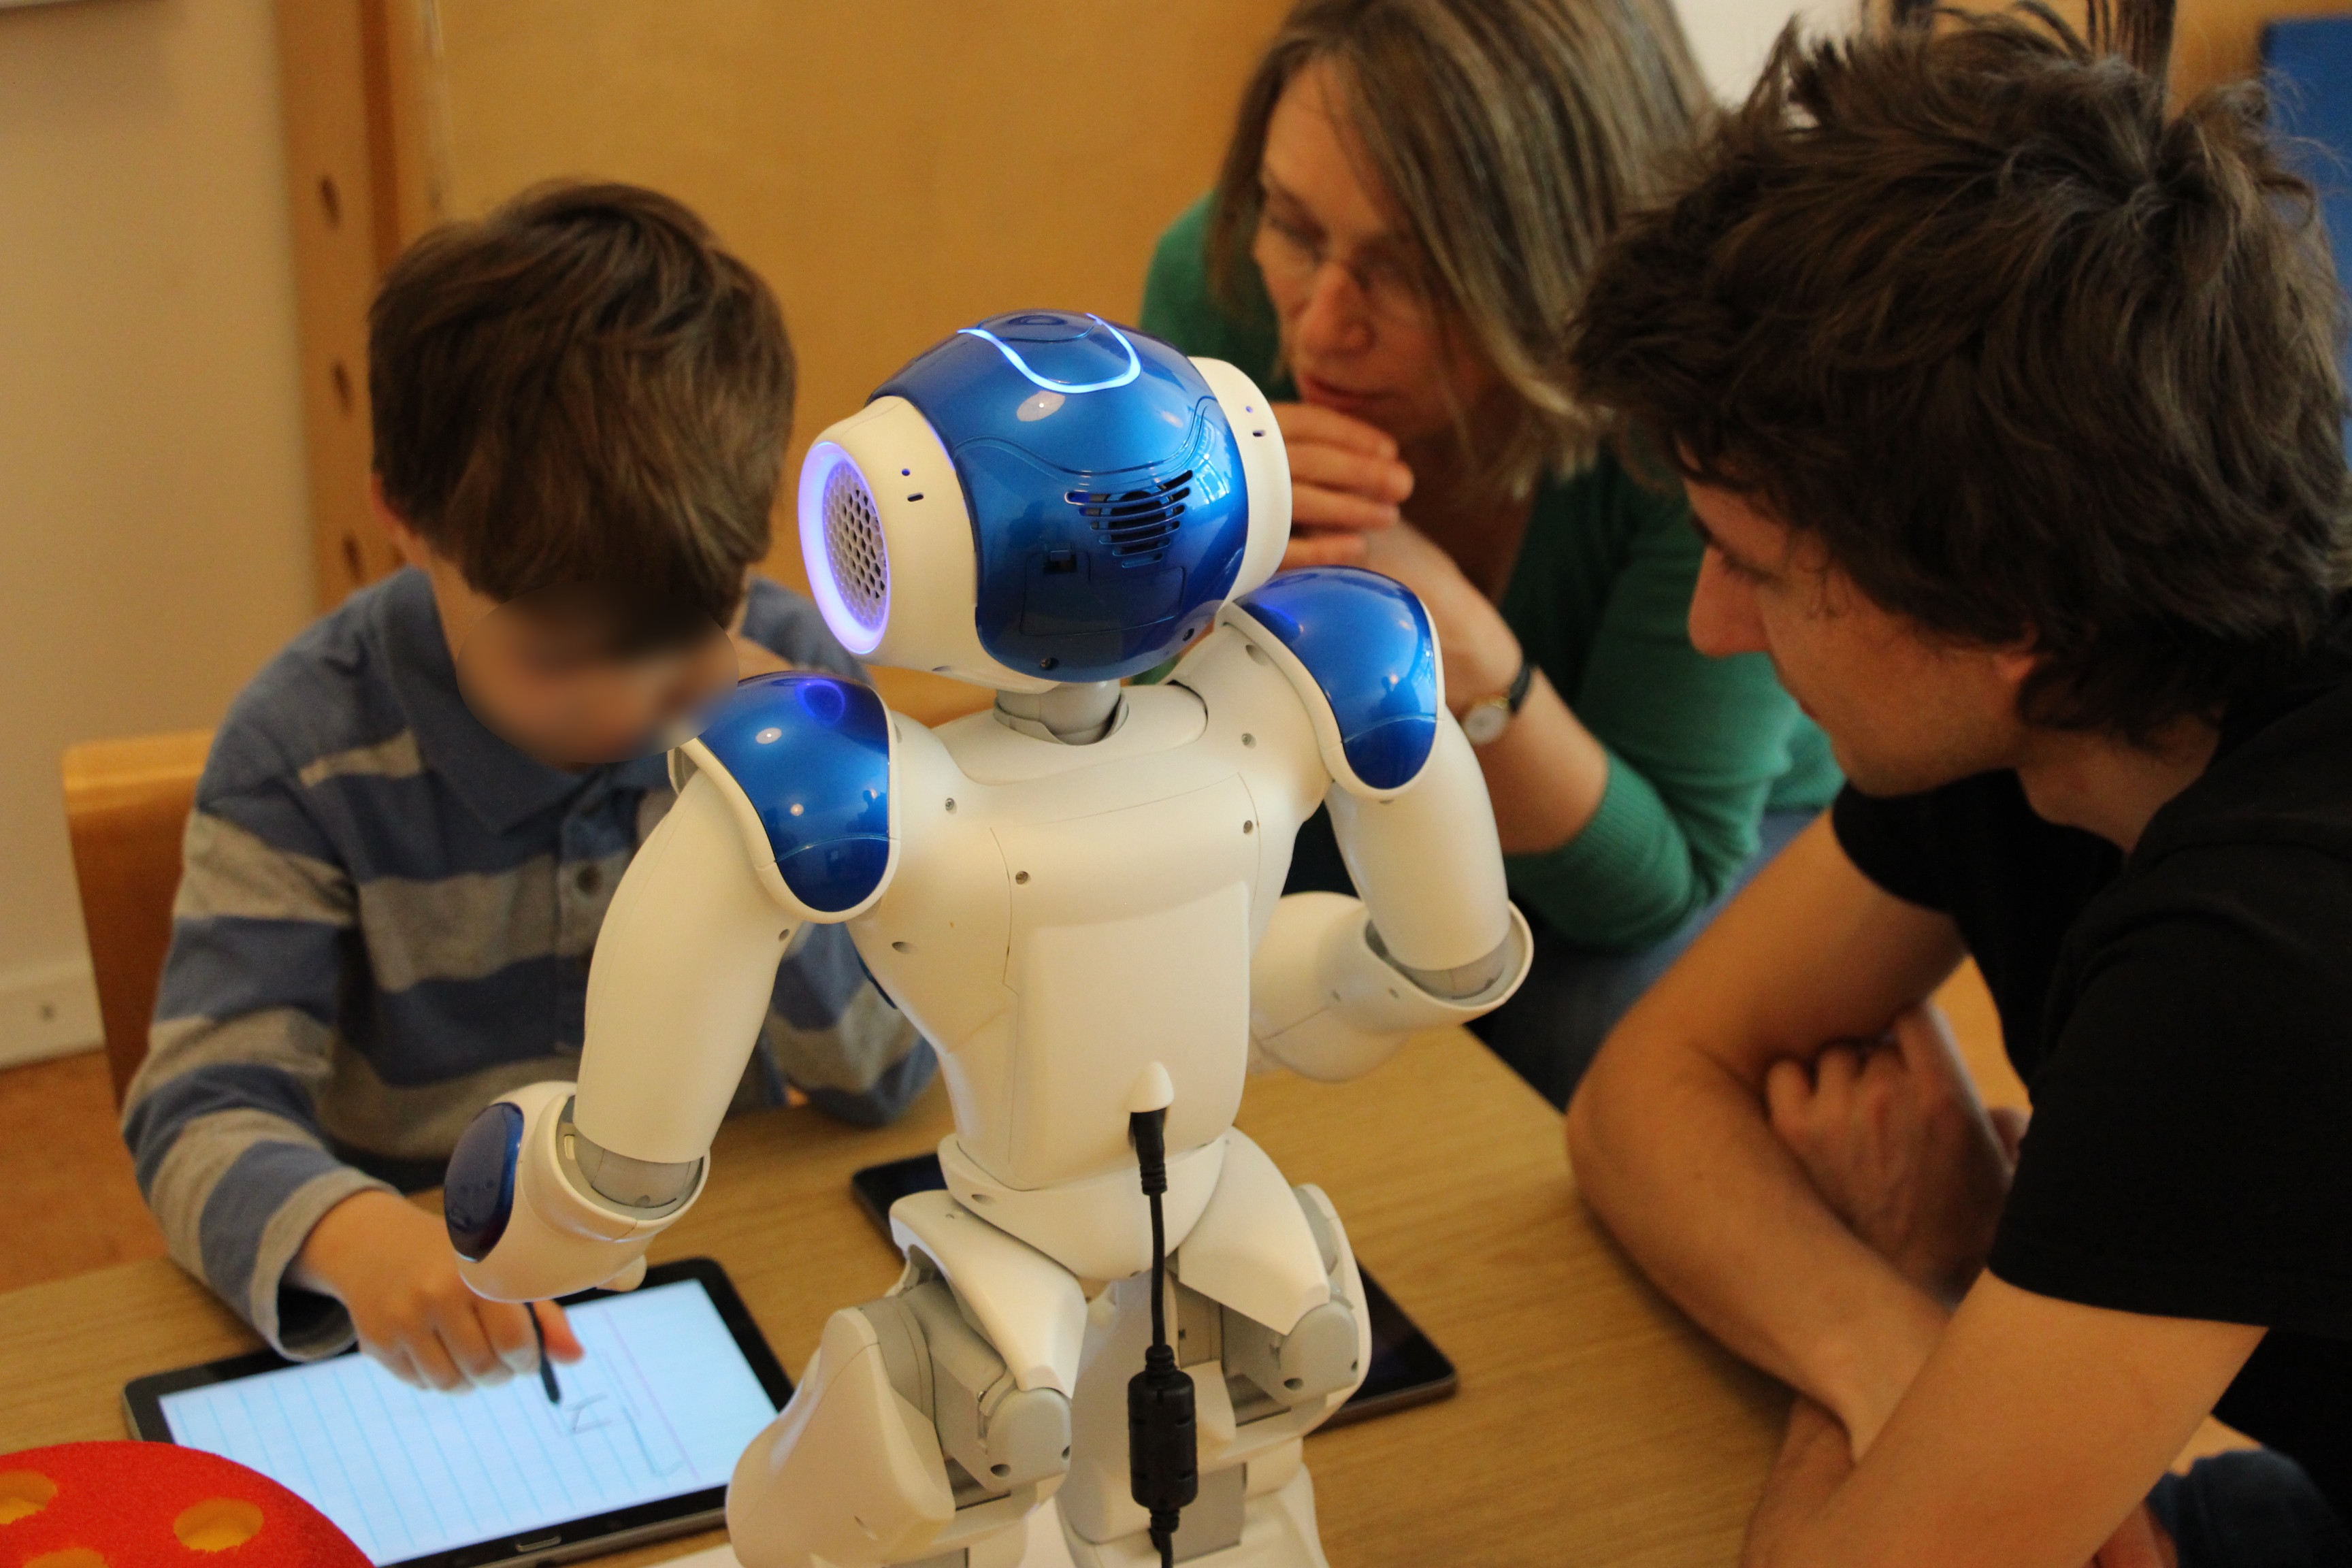
\includegraphics[width=0.9\linewidth]{henry}
%       \caption{Henry teaching Nao how to write numbers, with the help of an occupational therapist.}
%       \label{fig:henry}
%   \end{figure}

\section{case 1 : Diego}
Diego is a 5 years hold child. 
A few days before the experiment, his mother provided us with a picture showing
some of his handwriting works (figure~\ref{fig:diego_start}). 
This sample allowed us to create a dataset of letters based on his main mistake.
Then we run a PCA algorithm feed by this dataset to extract eigenvectors
representing the direction of the most important
deformations (figure~\ref{fig:3a}). 
Our idea was to use it to make the robot amplifying the mistakes of Diego. 
Thus, by correcting the robot, Diego was actually going to correct himself.    

\begin{figure}
    \centering
    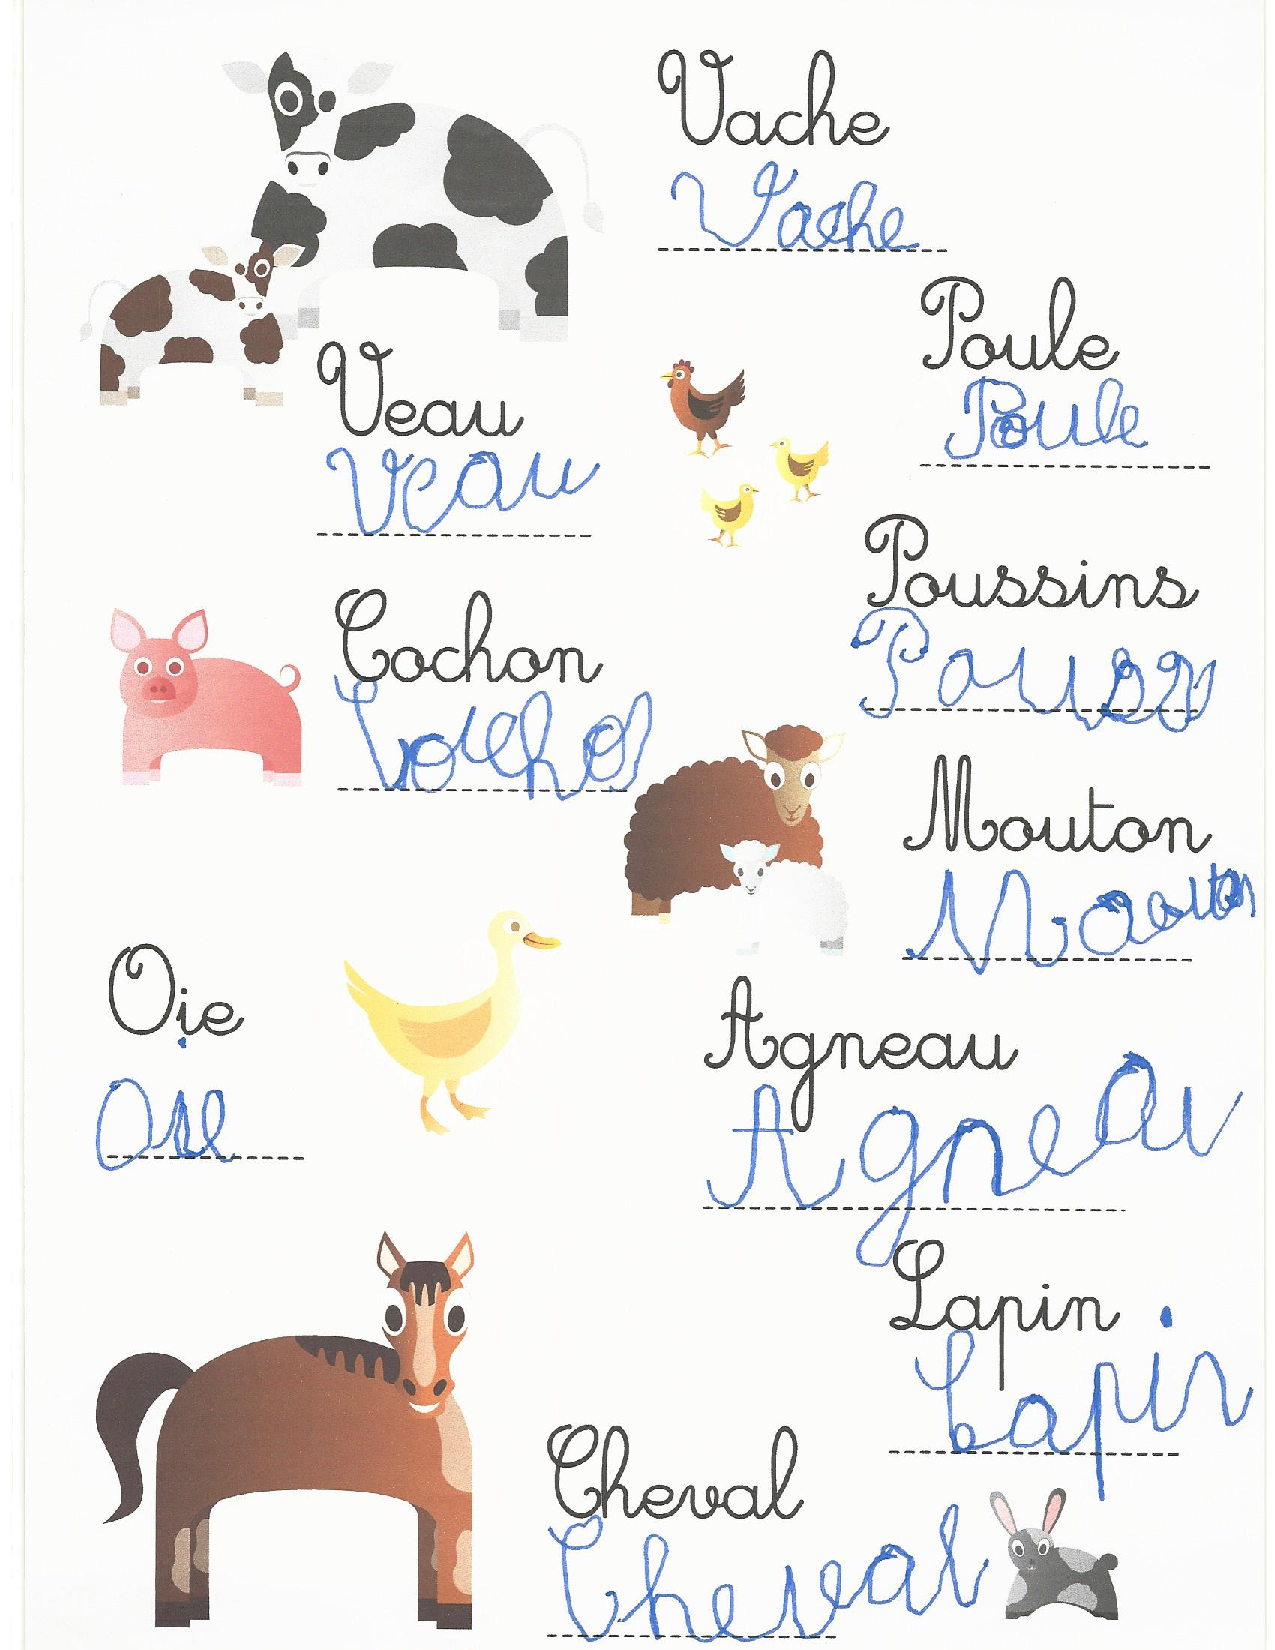
\includegraphics[width=0.9\linewidth]{diego_start}
    \caption{Homework performed by Diego before the experiment. It gives an
    overvew of his starting level in handwriting.}
    \label{fig:diego_start}
\end{figure}

\begin{figure}
    \centering
    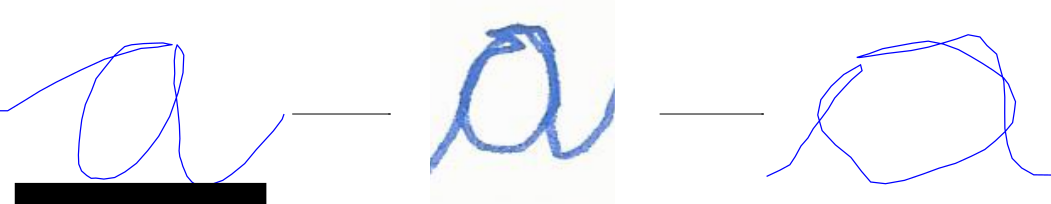
\includegraphics[width=0.9\linewidth]{3a}
    \caption{Letter deformation along an eigenvector. \emph{Left} : the non-deformed
        letter (origin of the eigenspace). \emph{Middle} : the actual Diego's
        deformation (from figure~\ref{fig:diego_start}). \emph{Right} : exaggerated
deformation along the eigenvector that encode Diego's mistake.} 
    \label{fig:3a}
\end{figure}

\subsection{Questions}
This was the first time we where trying a long-terme interaction between a child
and the CoWriter robot. So the first aim of this study was to see if such an
interaction was simply possible. If we could create an environement to keep a child engaged
during one hour just in writing words with the robot.
The second question was focused on the content of the interaction. Our goal was
to figure out what extent the child would actually improve the robot's writing. 

\subsection{Experimental settings}
The experiment took one month. It was divided in four sessions of one hour, one session per week.
In order to justify to the child an activity where a robot wants to learn
handwriting, we decided to adduce a scenario. There where two Nao robots: a
blue one (Mimi) and an orange one (Clem). They where introduced to the child as two hold friends. During the first
three sessions, Mimi was in "mission" : it was exploring a mysterious hidden
base. Each week, just before the session, it was sending a postal mail contening
a picture, a curious object it found and a few words about its discoveries. The pictures was representing itself exploring 
a dark room of the hidden base (that was actually our laboratory's workshop). 
The objects where 3D printed. In fact, there where puzzle pieces of a small 3D 
model of Nao robot but regarding them one by one, it was not easy to guess it.


%   \begin{figure}
%       \centering
%       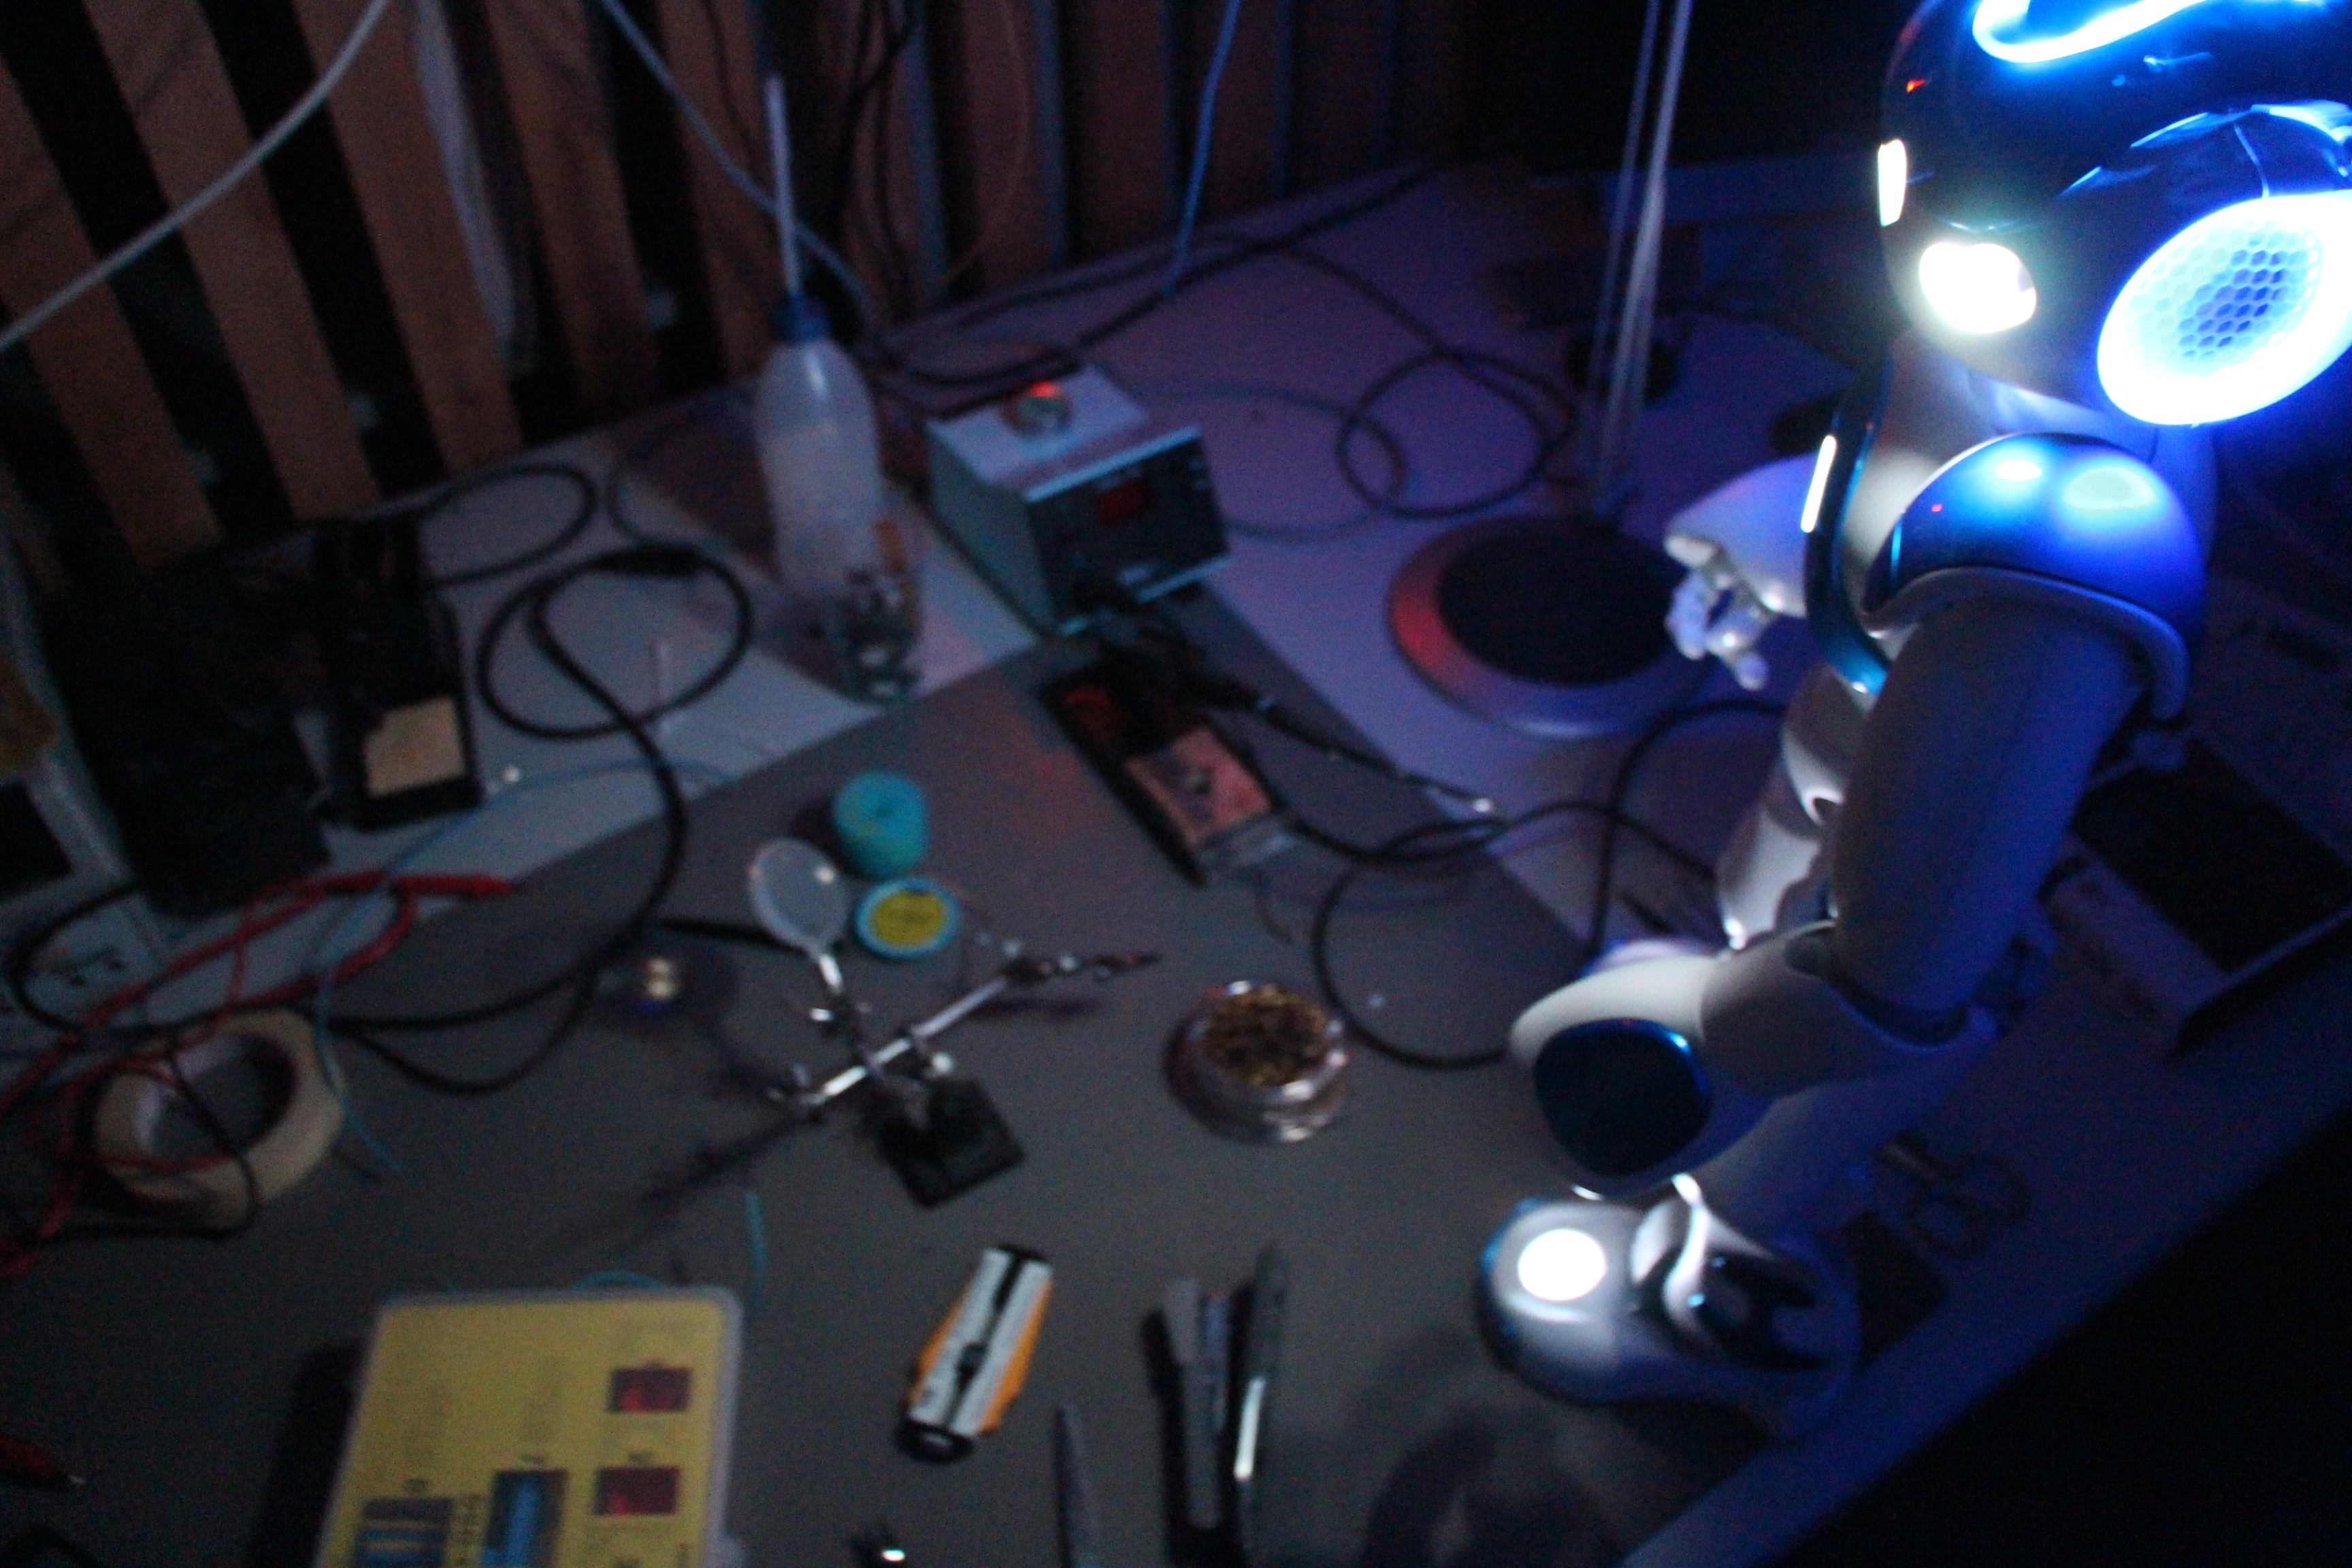
\includegraphics[width=0.9\linewidth]{mimi_mails}
%       \caption{Exemple of content of the mails sent by Mimi. A : pictures of Mimi exploring the
%           hidden base. B : some curious objects found by Mimi in the base. C :
%           few words about its adventures and discoveries.
%       }
%       \label{fig:mimi_mails}
%   \end{figure}


\subsection{Results}

\section{case 2 : Henry}
Description of experiments \& results with Diego

\subsection{Experiment design}

\subsection{Results}

\section{Discussion}

\section{Conclusions}

\bibliographystyle{abbrv}
\bibliography{cowriter} 
\end{document}
